%-------------------------------------------------------------------------
% CURIE Academy Design Project
%-------------------------------------------------------------------------

\documentclass{cbxdoc}

\usepackage{titletoc}

\usepackage{svg}

\dottedcontents{section}[2em]{\vspace{0.02in}}{1.5em}{0.7em}

\makeatletter
\renewcommand\tableofcontents{%
    \@starttoc{toc}%
}
\makeatother

%-------------------------------------------------------------------------
% Document Parameters
%-------------------------------------------------------------------------

\title{CURIE Academy, Summer 2014}
\subtitle{Design Project Input/Output Module Descriptions}

\institution
{%
  Prof. Christopher Batten \\
  School of Electrical and Computer Engineering \\
  Cornell University
}

%-------------------------------------------------------------------------
% Document
%-------------------------------------------------------------------------

\begin{document}

\maketitle

Each IoT design project will involve building an IoT system comprised of
an IoT input device, IoT cloud, and IoT output device. The IoT input
devices will have various input modules attached that can sense what is
going on in the environment (e.g., light, temperature, motion, force,
current, pulse, liquid) and be able to upload data into the cloud. Each
IoT output device will be able to download data from the could and will
have various output modules attached to display data (e.g., LEDs, piezo
buzzer, mini-printer) or react in some way (e.g., servo, relay for
controlling appliances). The following diagram illustrates the overall
approach we will be using in our IoT systems.

\begin{center}
  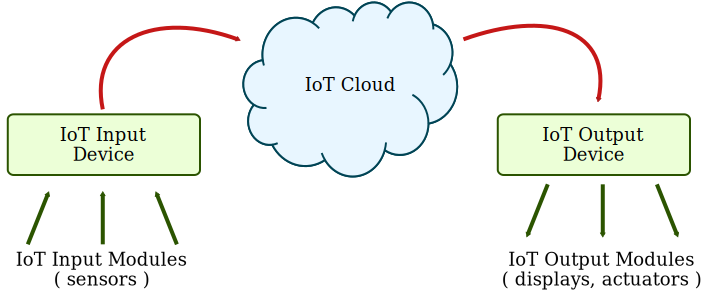
\includegraphics[width=0.75\tw]{curie-project-diagram.svg.pdf}
\end{center}

The rest of this document describes each input/output module and gives a
simple circuit along with the corresponding code to get you started. You
will need to work on your own to determine the best way to integrate the
input/output module with the IoT cloud. You can use Lab 3 as an example.
The various input and output modules are listed below.

\begin{center}\small
 \begin{minipage}{0.8\textwidth}
   \tableofcontents
 \end{minipage}
\end{center}

%-------------------------------------------------------------------------
% Design Project Input/Output Module Description
%-------------------------------------------------------------------------

\clearpage
\section{Light Input Module}
\label{sec-input-light}

This input module enables your IoT device to sense how much light is
reaching the device. The module uses a small photo-resistor which is
similar in spirit to the potentiometer you experimented with in Lab~2.
For the potentiometer, the resistance varied as you twisted the knob on
the robot. For the photo-resistor, the resistance will vary based on how
much light reaches the device. The Arduino cannot directly sense
resistance, but it can sense an analog input voltage. We will use a
simple circuit called a voltage divider so that the voltage across the
photo-resistor is proportional to the resistance.

A sample circuit and Arduino code is shown below to get you started. The
circuit places a \wu{10}{k$\Omega$} resistor in series with the
photo-resistor. A \wu{10}{k$\Omega$} resistor has brown-black-orange
bands. We use a wire to connect the node in between the resistor and the
photo-resistor to an analog input of the Arduino. The example code will
print the analog reading from the photo-resistor on the serial monitor,
similar to how we printed the analog reading from the grayscale sensor in
Lab~2. After setting up the circuit and programming the Arduino, open the
serial monitor and note how the sensor reading varies when the device is
covered with your hand or when the device is placed under a bright light.
The reading from the sensor should get larger when the device is in a
dark environment, and should get smaller when the device is in a bright
environment.

\vspace{0.1in}
\begin{minipage}[t]{0.49\tw}
  \vspace{0pt}

  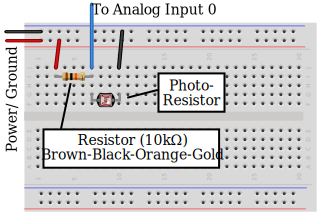
\includegraphics[width=\tw]{input-light-annotated.svg.pdf}
\end{minipage}
\hfill
\begin{minipage}[t]{0.49\tw}
  \vspace{0.1in}
  \begin{Verbatim}[gobble=3,fontsize=\small]
    int pin_light = 5;

    void setup() {
      Serial.begin(9600);
    }

    void loop() {
      int light_level = analogRead( pin_light );
      Serial.println( light_level );
      delay(1000);
    }
  \end{Verbatim}
\end{minipage}


%-------------------------------------------------------------------------
% Design Project Input/Output Module Description
%-------------------------------------------------------------------------

\section{Infrared (IR) Input Module}
\label{sec-input-ir}

% What it does at a high level
This input module enables your IoT device to sense the distance of an
object placed \wu{10-80}{cm} in front of it, using the same Sharp
GP2Y0A21 Distance Sensor you experimented with in your robot in Lab 2.
The sensor works by bouncing infrared (IR) light off objects and sensing
the angle at which it returns -- a process called \IT{triangulation}.
The output of the sensor is a distance, derived from the angle of
reflected light.

A sample circuit and Arduino code is shown below to get you started.
This code will print the analog reading from the IR sensor on the serial
monitor, similar to how we printed the analog reading from the grayscale
sensor in Lab 2. After setting up the circuit and programming the
Arduino, open the serial monitor and experiment with placing objects
(e.g., a book) at various distances away from the front of the sensor.
The reading from the sensor should be larger for objects farther away
from the sensor and smaller for objects closer to the sensor.

% Questions:
% 1) What happens if the object is further than 80cm (max range) from the sensor?
% 2) What happens if the object is closer than 10cm (min range) from the sensor?
% 3) The sensor is not outputting distance in any particular unit. Can
% you make it output distance in centimeters?

\vspace{0.1in}
\begin{minipage}[t]{0.49\tw}
  \vspace{0pt}

  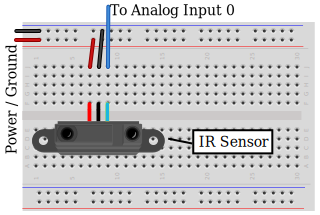
\includegraphics[width=\tw]{input-ir-annotated.svg.pdf}
\end{minipage}
\hfill
\begin{minipage}[t]{0.49\tw}
  \vspace{0.1in}
  \begin{Verbatim}[gobble=3,fontsize=\small]
    int pin_ir = 0;

    void setup() {
      Serial.begin(9600);
      pinMode( pin_ir, INPUT );
    }

    void loop() {
      int distance = analogRead( pin_ir );
      Serial.println( distance );
      delay(1000);
    }
  \end{Verbatim}
\end{minipage}


%-------------------------------------------------------------------------
% Design Project Input/Output Module Description
%-------------------------------------------------------------------------

\clearpage
\section{Temperature Input Module}
\label{sec-input-temperature}

This input module enables your IoT device to sense the temperature of
the environment using an easy-to-use temperature sensor. This may be
useful in environmental control systems, thermal protection, industrial
process control, fire alarms, power system monitors, cpu thermal
management, etc. The TMP36 temperature sensor contains an integrated
circuit with a single signal output lead. This signal's voltage rises
and falls, depending on the ambient temperature, at \wu{10}{mV} per
degree centigrade (Celsius).

A sample circuit and Arduino code is shown below to get you started.
There is no need for any extra components; we directly connect the
middle lead on the temperature sensor to an analog input on the Arduino.
Make sure the sensor's "flat end" is facing the correct direction (shown
in the diagram). If you point the flat end of the sensor to your left,
the top lead connects to power (the red wire), the middle lead is the
signal, and the bottom lead connects to ground (the black wire).

Since the analog reading from the temperature sensor is a digital value
between 0 and 1023, the example code scales this value to a range
between \wu{0--5}{V}, converts voltage to temperature, and then prints
the temperature in centigrade (Celsius) on the serial monitor, similar
to how we printed the analog reading from the grayscale sensor in Lab~2.
After setting up the circuit and programming the Arduino, open the
serial monitor and check the reported room temperature in degrees
centigrade (Celsius). Does the reading sound right? Experiment with the
sensor by changing the ambient temperature (e.g., with a hair dryer)
and see how warm or cool you can make it!

\vspace{0.1in}
\begin{minipage}[t]{0.49\tw}
  \vspace{0.6in}

  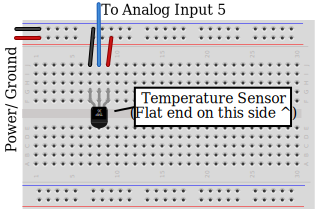
\includegraphics[width=\tw]{input-temperature-annotated.svg.pdf}
\end{minipage}
\hfill
\begin{minipage}[t]{0.49\tw}
  \vspace{0.1in}
  \begin{Verbatim}[gobble=3,fontsize=\small]
    int pin_temperature = A0;

    void setup() {
      Serial.begin(9600);
      pinMode( pin_temperature, INPUT );
    }

    void loop() {

      // Read temperature sensor and convert from
      // a 0 to 1023 digital range to 0 to 5 volts.

      float voltage =
        analogRead( pin_temperature ) * .004882814;

      // Convert from 10 mV per degree with 500
      // mV offset to degrees Celsius (i.e.,
      // temperature = (voltage-500mV) * 100).

      float temperature = (voltage - .5) * 100;

      Serial.println( temperature );
      delay(1000);
    }
  \end{Verbatim}
\end{minipage}
\vspace{0.1in}

%Questions:

%-------------------------------------------------------------------------
% Design Project Input/Output Module Description
%-------------------------------------------------------------------------

\clearpage
\section{Force Input Module}
\label{sec-input-force}

% FIXME: replace 'force' with 'pressure'? or leave them all 'force'?

This input module enables your IoT device to sense the amount of force
exerted on the surface of a pressure pad. The sensor is a resistor with
a resistance that varies depending on how much force is exerted on the
pressure pad (e.g., by squeezing it between two fingers); the resistance
is high (infinite) when there is no pressure and low when the pressure
is high. The Arduino cannot directly sense resistance, but we can set up
a voltage divider so that the Arduino can sense voltage instead. This
way, as we apply more pressure to the sensor, the voltage the Arduino
reads decreases.

% FIXME: replace 'ohm' with symbol..

A sample circuit and Arduino code is shown below to get you started.
The voltage divider circuit is formed by the force sensor and the
\wu{10}{kohm} resistor, and the Arduino reads the voltage from one end
of the resistor to ground. The example code will print the analog
reading from the force sensor on the serial monitor, similar to how we
printed the analog reading from the grayscale sensor in Lab~2. After
setting up the circuit and programming the Arduino, open the serial
monitor and check the value the force sensor is detecting. Then try
squeezing the pressure pad between two fingers and see the reading
increase.

\vspace{0.1in}
\begin{minipage}[t]{0.49\tw}
  \vspace{0pt}

  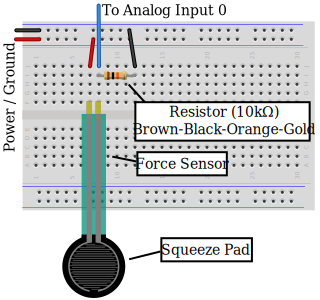
\includegraphics[width=\tw]{input-force-annotated.svg.pdf}
\end{minipage}
\hfill
\begin{minipage}[t]{0.49\tw}
  \vspace{0.1in}
  \begin{Verbatim}[gobble=3,fontsize=\small]
    int pin_force = 0;

    void setup() {
      Serial.begin(9600);
      pinMode( pin_force, INPUT );
    }

    void loop() {
      int force = analogRead( pin_force )

      Serial.println( force );
      delay(1000);
    }
  \end{Verbatim}
\end{minipage}
\vspace{0.1in}

%Questions:

%-------------------------------------------------------------------------
% Design Project Input/Output Module Description
%-------------------------------------------------------------------------

\clearpage
\section{Flex Input Module}
\label{sec-input-flex}

This input module enables your IoT device to sense the flexing of a
\wu{6}{cm} strip. The flex sensor is a resistor with a resistance that
varies depending on how much the strip is flexed (e.g., by bending it);
the resistance is higher when flexed in one direction and lower when
flexed in the other. The Arduino cannot directly sense resistance, but
we can set up a voltage divider so that the Arduino can sense voltage
instead. This way, as we flex the sensor, the voltage the Arduino reads
changes accordingly.

% FIXME: replace 'ohm' with symbol..

A sample circuit and Arduino code is shown below to get you started.
The voltage divider circuit is formed by the flex sensor and the
\wu{10}{kohm} resistor, and the Arduino reads the voltage from one end
of the resistor to ground. The example code will print the analog
reading from the flex sensor on the serial monitor, similar to how we
printed the analog reading from the grayscale sensor in Lab~2. After
setting up the circuit and programming the Arduino, open the serial
monitor and check the value the flex sensor is detecting. Then try
flexing the sensor strip in either direction and see the reading
increase and decrease accordingly.

\vspace{0.1in}
\begin{minipage}[t]{0.49\tw}
  \vspace{0pt}

  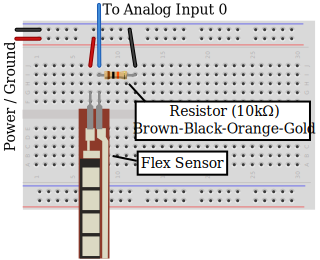
\includegraphics[width=\tw]{input-flex-annotated.svg.pdf}
\end{minipage}
\hfill
\begin{minipage}[t]{0.49\tw}
  \vspace{0.1in}
  \begin{Verbatim}[gobble=3,fontsize=\small]
    int pin_flex = 0;

    void setup() {
      Serial.begin(9600);
      pinMode( pin_flex, INPUT );
    }

    void loop() {
      int flex = analogRead( pin_flex );

      Serial.println( flex );
      delay(1000);
    }
  \end{Verbatim}
\end{minipage}
\vspace{0.1in}

%Questions:

%-------------------------------------------------------------------------
% Design Project Input/Output Module Description
%-------------------------------------------------------------------------

\clearpage
\section{Water Input Module}
\label{sec-input-water}

This input module enables your IoT device to sense the level of water in
the environment using a water sensor called eTape. Water level sensing
can play an important role in environmental monitoring systems, disaster
warning, cooling systems, water purification, medical equipment care,
etc. This tape can easily be secured to a street pole, hung on the wall
of a room, or attached to the side of a water container or other similar
environments. The tape is a variable resistor. When immersed in water,
the sensor tape is compressed from both sides by hydrostatic pressure,
and the tape's resistance varies as the water level rises and falls. The
resistance and water level are inversely proportional: the lower the
water level, the higher the output resistance; the higher the water
level, the lower the output resistance.  The Arduino cannot directly
sense resistance, but it can sense an analog input voltage. We will use
a simple circuit called a voltage divider so that the voltage across the
water sensor is proportional to the resistance.

A sample circuit and Arduino code is shown below to get you started.
The circuit places a \wu{560}{$\Omega$} resistor in series with the
water sensor so that voltage is divided between the two components. A
\wu{560}{$\Omega$} resistor has green-blue-purple bands. We use a wire
to connect the node in between the resistor and the water sensor to an
analog input of the Arduino so that the Arduino can read the voltage
from one end of the \wu{560}{$\Omega$} resistor to ground. Use long
wires to connect the water sensor to the breadboard so that you can
freely move the sensor away from the Arduino and breadboard (which
should not get wet!). The example code will print the analog reading
from the water level sensor on the serial monitor, similar to how we
printed the analog reading from the grayscale sensor in Lab~2. After
setting up the circuit and programming the Arduino, open the serial
monitor and check the value of the water level sensor when dipped in a
container of water. Be careful not to get the top electrical leads of
the sensor wet. Try dipping the water level sensor further into the
water. What happens to the reading and why do you think this happens?

\vspace{0.1in}
\begin{minipage}[t]{0.49\tw}
  \vspace{0pt}

  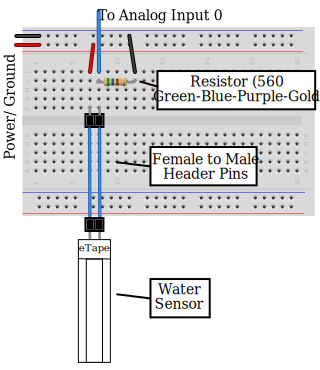
\includegraphics[width=\tw]{input-water-annotated.svg.pdf}
\end{minipage}
\hfill
\begin{minipage}[t]{0.49\tw}
  \vspace{0.1in}
  \begin{Verbatim}[gobble=3,fontsize=\small]
    int pin_water = A0;

    void setup() {
      Serial.begin(9600);
      pinMode( pin_water, INPUT );
    }

    void loop() {
      int water_level = analogRead( pin_water )

      Serial.println( water_level );
      delay(1000);
    }
  \end{Verbatim}
\end{minipage}
\vspace{0.1in}

%Questions:

%-------------------------------------------------------------------------
% Design Project Input/Output Module Description
%-------------------------------------------------------------------------

\clearpage
\section{Accelerometer Input Module}
\label{sec-input-accel}

This input module enables your IoT device to sense physical acceleration
-- perfect for applications requiring tilt-sensing, motion, shock,
vibration, etc. The ADXL335 3-axis accelerometer you will use is a
micro-electro-mechanical system (MEMS) device: a device that combines
tightly-coupled electrical and mechanical systems on a very small scale
(micro-meters!). The accelerometer works by measuring the capacitance
between fixed plates and a tiny structure suspended in mid-air by tiny
springs. As the device experiences acceleration in the X, Y, and/or Z
axes, the suspended structure deflects, changing the capacitance along
each axis. Each capacitance converts to an output voltage, proportional
to the acceleration on that axis, which can then be sensed by the
Arduino.

A sample circuit and Arduino code is shown below to get you started.
The example code will print calibrated accelerometer readings for each
axis on the serial monitor, similar to how we printed the analog reading
from the grayscale sensor in Lab~2. After setting up the circuit and
programming the Arduino, open the serial monitor, place your device on
the table, and check the values the accelerometer is sensing. These
should be close to (x = 0, y = 0, z = 100). Then pick up the device and
tilt it or shake it. See how the values change along the three axes!

\vspace{0.1in}
\begin{minipage}[t]{0.49\tw}

  \vspace{0.0in}
  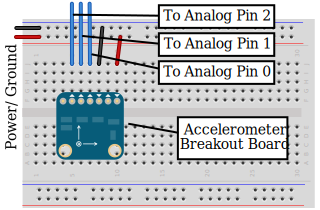
\includegraphics[width=\tw]{input-accel-annotated.svg.pdf}

  \vspace{0.0in}
  \begin{Verbatim}[gobble=3,fontsize=\small]
    int pin_x_accel = A2;
    int pin_y_accel = A1;
    int pin_z_accel = A0;

    // Calibration

    int x_min = 267; int x_max = 399;
    int y_min = 272; int y_max = 404;
    int z_min = 274; int z_max = 412;

    void setup() {
      Serial.begin(9600);
    }
  \end{Verbatim}
\end{minipage}
\hfill
\begin{minipage}[t]{0.49\tw}
  \vspace{0.0in}
  \begin{Verbatim}[gobble=3,fontsize=\small]
    void loop() {
      // Read each axis.

      int x_raw = analogRead( pin_x_accel );
      int y_raw = analogRead( pin_y_accel );
      int z_raw = analogRead( pin_z_accel );

      // Scale measurements to calibrated minimum
      // and maximum.

      int x_scaled =
        map( x_raw, x_min, x_max, -100, 100 );
      int y_scaled =
        map( y_raw, y_min, y_max, -100, 100 );
      int z_scaled =
        map( z_raw, z_min, z_max, -100, 100 );

      // Report scaled measurements.

      Serial.print("  x: "); Serial.print( x_scaled );
      Serial.print("; y: "); Serial.print( y_scaled );
      Serial.print("; z: "); Serial.print( z_scaled );
      Serial.println();

      // Wait 500ms before next reading.

      delay(500);
    }
  \end{Verbatim}
\end{minipage}
\vspace{0.1in}

%Questions:

%-------------------------------------------------------------------------
% Design Project Input/Output Module Description
%-------------------------------------------------------------------------

\clearpage
\section{RF Input Module}
\label{sec-input-rf}

This input module enables your IoT device to send and receive radio
frequency (RF) signals wirelessly in a \wu{25}{ft} radius. RF control
devices are useful in many applications -- e.g., car security systems,
home security and automation systems, garage door controllers, remote
control fan, remote control toys, remote control industrial use. In an
RF-based control system, an RF transmitter sends signals -- radio waves
in the range of \wu{3}{kHz} to \wu{300}{GHz} -- and an RF receiver
receives the signals and can then act on them. In this module, you will
use a 4-button keyfob RF remote to send \wu{315}{MHz} signals to an RF
receiver connected to your Arduino, which can then act on the signal.

A sample circuit is shown below to get you started. If you look closely
at the RF receiver module, you will see that it has seven pins total.
Besides power and ground, the D0, D1, D2, and D3 pins are signal pins
corresponding to the four buttons on the keyfob RF remote; VT is a
special pin that is true if any button is pushed and false if none are
pushed. Connect D0, D1, D2, and D3 to the analog input pins on the
Arduino. The 4-button keyfob RF remote requires no assembly or
connectivity. It has four buttons that are labeled "A", "B", "C", and
"D". Pressing any of these transmits a \wu{315}{MHz} radio wave command
to be picked up by the RF receiver.

The example Arduino code shown below will read which button you have
pressed on the remote, and then print the output on the serial monitor,
similar to how we printed the analog reading from the grayscale sensor
in Lab~2. The printout refreshes every \wu{100}{ms}. After setting up the
circuit and programming the Arduino, open the serial monitor and try
pressing each button on the RF remote. You should see each letter
detected by the Arduino displayed on the serial monitor. Try to see how
far away you can move with the RF remote while still successfully
receiving the signal!

\vspace{0.1in}
\begin{minipage}[t]{0.49\tw}

  \vspace{0.1in}
  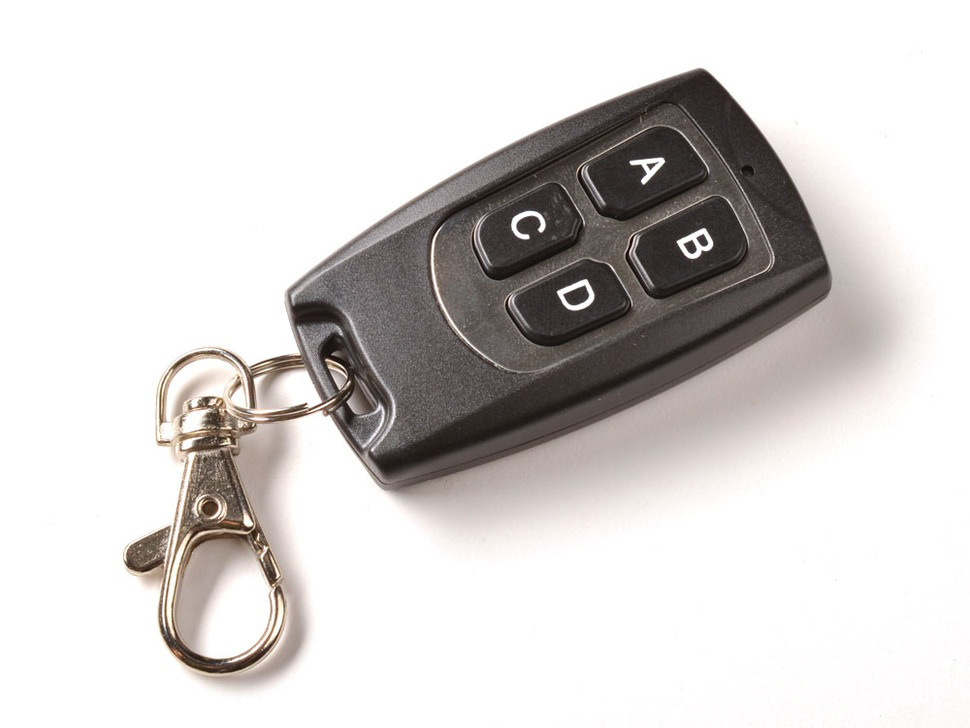
\includegraphics[width=\tw]{rf-remote.jpg}

  \vspace{0.1in}
  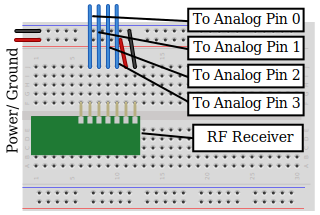
\includegraphics[width=\tw]{input-rf-annotated.svg.pdf}

\end{minipage}
\hfill
\begin{minipage}[t]{0.49\tw}
  \vspace{0.1in}
  \begin{Verbatim}[gobble=3,fontsize=\small]
    int pin_RF_A = 3;
    int pin_RF_B = 6;
    int pin_RF_C = 7;
    int pin_RF_D = 10;

    void setup() {
      pinMode( pin_RF_A, INPUT );
      pinMode( pin_RF_B, INPUT );
      pinMode( pin_RF_C, INPUT );
      pinMode( pin_RF_D, INPUT );
      Serial.begin(9600);
    }

    void loop() {

      // Read RF input on each pin

      int A = digitalRead( pin_RF_A );
      int B = digitalRead( pin_RF_B );
      int C = digitalRead( pin_RF_C );
      int D = digitalRead( pin_RF_D );

      // Print the letter if the input is detected.
      // Otherwise, print '-' if nothing is detected.

      if (A) Serial.print("A"); else Serial.print("-");
      if (B) Serial.print("B"); else Serial.print("-");
      if (C) Serial.print("C"); else Serial.print("-");
      if (D) Serial.print("D"); else Serial.print("-");

      // After checking all four inputs, make a new line.

      Serial.println();

      // Loop every 100ms.

      delay(100);
    }
  \end{Verbatim}
\end{minipage}
\vspace{0.1in}

%Questions:


%-------------------------------------------------------------------------
% Design Project Input/Output Module Description
%-------------------------------------------------------------------------

\clearpage
\section{emonTx Power Input Module}
\label{sec-input-power}

This input module enables your IoT device to read the AC voltage and current
used to power lights, appliances, and everything else in your home.  The emonTx
Shield you will use was developed by the Open Energy Monitoring group out of the
UK and is designed to ``create a fully open-source energy monitoring and control
system that is suitable for domestic and industrial application.''  

The emonTx will allow you to interface your Arduino's Analog-to-Digital
Converters (ADCs) to current and voltage sensors.  This enables you to safely
measure the voltage and current that a lamp, for example, uses when plugged into
the wall.  You will be using an AC-to-AC adapter to measure voltage. Using a
transformer, the AC-to-AC adapter reduces the wall voltage down by a factor of
about 12, so 110V becomes 9V.  If the wall voltage changes, you will be able to
see that change, reduced by a factor of about 12.  The current sensor is also a
transformer.  By wrapping a ferrite loop around a wire, you can detect the
induced magnetic field from an AC current in the wire.  This induced field
creates a voltage proportional to the current, which we can measure using the
Arduino.  Power is current times voltage, or $P=IV$, so armed with these two
measurements we can calculate the power in watts consumed by a household device.

A sample circuit and Arduino code is shown below to get you started.  
The emonTx plugs directly into the Arduino, the current sensors plug into the
3.5mm audio jacks, and the AC-to-AC connector goes into the barrel connector
jack.  We will share the voltage sensor across all of the current sensors (note
that current sensor 4 is disabled, so don't use it).  The sample code below will
let you calculate power for the devices connected to current sensor 1.

\vspace{0.1in}
\begin{minipage}[t]{0.49\tw}

  \vspace{0.1in}
    Picture goes here!

\end{minipage}
\hfill
\begin{minipage}[t]{0.49\tw}
  \vspace{0.1in}
  \begin{Verbatim}[gobble=3,fontsize=\small]
    // EmonLibrary examples openenergymonitor.org, Licence GNU GPL V3

    #include "EmonLib.h"             // Include Emon Library
    EnergyMonitor emon1;             // Create an instance

    float power_offset = 3.9;        // Include an offset to "zero" the power


    void setup()
    {  
      Serial.begin(9600);
      
      emon1.voltage(0, 120.0, 1.7);  // Voltage: input pin, calibration, phase_shift
      emon1.current(1, 60.6);       // Current: input pin, calibration.
    }

    void loop()
    {
      emon1.calcVI(20,2000);         // Calculate all. No.of half wavelengths
    (crossings), time-out
      float realPower       = emon1.realPower - power_offset;        //extract Real
    Power into variable
      float supplyVoltage   = emon1.Vrms;             //extract Vrms into Variable
      
      // Floor the power at 0 
      if (realPower < 0.0)
        realPower = 0.0;

      Serial.print(realPower); Serial.print("W @ "); 
      Serial.print(emon1.Vrms); Serial.println("V");
    }
  \end{Verbatim}
\end{minipage}
\vspace{0.1in}

%Questions:

%-------------------------------------------------------------------------
% Design Project Input/Output Module Description
%-------------------------------------------------------------------------

\clearpage
\section{Heart Rate Input Module}
\label{sec-input-heart}

This input module enables your IoT device to sense your heart beating.
Heart rate monitors are useful for monitoring heart rate in a variety of
applications, including exercise and fitness (targetting a healthy heart
rate), injury rehabilitation, hospital monitoring systems, and
biotelemetry. The Polar T34 Non-Coded Heart Rate Transmitter (the
wearable chest strap) monitors and then wirelessly transmits your heart
rate data from the chest strap to the Polar Heart Rate Receiver (the
small green IC), which can then communicate data to the Arduino. The
heart rate monitor works by detecting electrical heart muscle signals as
the heart beats. The chest strap can sense these electric signals when
the two contacts are moistened and are in direct contact with your skin,
and it sends a pulsed wireless signal to the receiver when it detects a
beat.

A sample circuit and Arduino code is shown below to get you started.
There is no need for any extra components. The example code will print
"Heartbeat" on the serial monitor whenever a heart beat is detected.
After setting up the circuit and programming the Arduino, you can secure
the chest strap to your partner's chest, just below the chest muscles,
and buckle the strap together. Moisten the two grooved electrode areas
on the back of the chest strap. Check that the wet grooved areas are
firmly against the skin and that the word "Polar" is right-side up. The
moistened grooved areas activate the transmitter, so make sure to dry
the sensor when not in use. After securing the chest strap, open the
serial monitor, use your hand to find your own pulse, and verify that
"Heartbeat" is printed at the same time your heart is beating.

\vspace{0.1in}
\begin{minipage}[t]{0.49\tw}
  \vspace{0pt}
  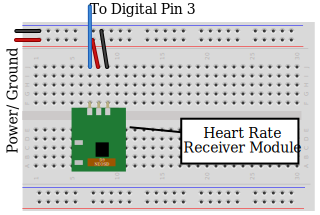
\includegraphics[width=\tw]{input-heart-annotated.svg.pdf}

  \vspace{0pt}
  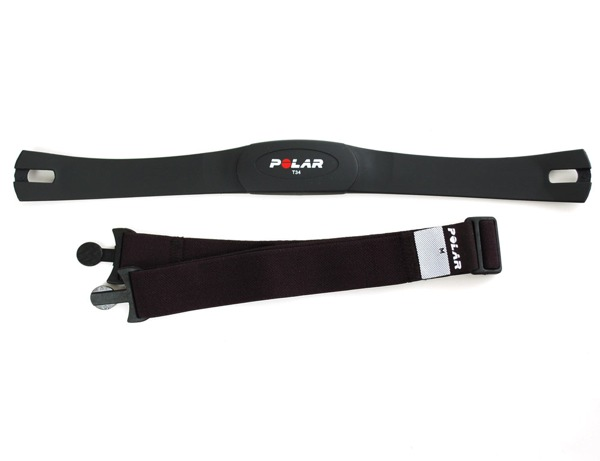
\includegraphics[width=\tw]{heart.jpg}
\end{minipage}
\hfill
\begin{minipage}[t]{0.49\tw}
  \vspace{0.1in}
  \begin{Verbatim}[gobble=3,fontsize=\small]
    int pin_heart = 3;
    byte oldSample, sample;

    void setup() {
      Serial.begin(9600);
      pinMode (pin_heart, INPUT);

      Serial.println("Waiting for heart beat...");

      // Wait until a heart beat is detected
      while ( !digitalRead(pin_heart) ) {};
      Serial.println ("Heart beat detected!");
    }

    void loop() {
      sample = digitalRead(pin_heart);
      if (sample && (oldSample != sample)) {
        Serial.println("Heartbeat");
      }
      oldSample = sample;
    }

  \end{Verbatim}
\end{minipage}


%-------------------------------------------------------------------------
% Design Project Input/Output Module Description
%-------------------------------------------------------------------------

\clearpage
\section{RGB LED Output Module}
\label{sec-output-rgb}

This output module enables your IoT device to display colored light
using an RGB LED (three LEDs in a single housing), where RGB stands for 'red',
'green', and 'blue'. Using the RGB LED, we can generate any color we
desire through color mixing. Do you remember color wheels from
elementary school?

A sample circuit and Arduino code is shown below to get you started.
Three leads of the RGB LED are set by digital output Arduino pins
corresponding to 'red', 'green', and 'blue'; the longest lead of the RGB
LED provides power. The example code will set the color of the RGB LED
to violet. After setting up the circuit and programming the Arduino,
check to make sure the RGB LED lights up violet. You can then experiment
with other colors by choosing your own RGB values (the table below lists
RGB values for common colors), and if you like, you can also try to make
the LED blink or change colors in time.

\vspace{0.1in}
\begin{minipage}[t]{0.49\tw}
  \vspace{0pt}

  \centering
    \begin{tabular}{l|l}
    \BF{Color} & \BF{RGB values} \\\hline
    RED     & (255, 0, 0) \\
    ORANGE  & (83, 4, 0) \\
    YELLOW  & (255, 255, 0) \\
    GREEN   & (0, 255, 0) \\
    BLUE    & (0, 0, 255) \\
    INDIGO  & (4, 0, 19) \\
    VIOLET  & (23, 0, 22) \\
    CYAN    & (0, 255, 255) \\
    MAGENTA & (255, 0, 255) \\
    WHITE   & (255, 255, 255) \\
    PINK    & (158, 4, 79) \\
    \end{tabular}
  \centering

  \vspace{0pt}

  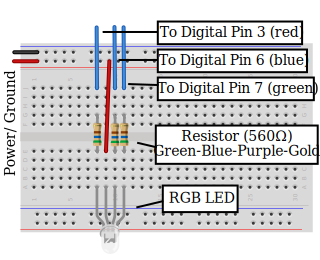
\includegraphics[width=\tw]{output-rgb-annotated.svg.pdf}
\end{minipage}
\hfill
\begin{minipage}[t]{0.49\tw}
  \vspace{0.1in}
  \begin{Verbatim}[gobble=3,fontsize=\small]
    // Choose RGB LED pins (these must be PWM pins)
    // redPin = 3, greenPin = 5, bluePin = 6
    int pin_RGB[] = {3, 5, 6};

    void setup() {
      for (int i = 0; i < 3; i++) {
        pinMode( pin_RGB[i], OUTPUT );
      }
    }

    void loop() {
      // Choose the RGB (red, green, blue) value
      // In this demo, we choose violet.

      byte my_color[] = {23, 0, 22};

      // Iterate through each of the three pins
      // (red, green blue).

      for (int i = 0; i < 3; i++) {

        // Write the analog value to the pin. We
        // use (255 - value) because our RGB LED
        // is common anode, which means the color
        // is fully on when we output
        // analogWrite( pin, 0 ) and fully off when
        // we output analogWrite( pin, 255).

        analogWrite( pin_RGB[i], 255 - my_color[i] );
      }
    }
  \end{Verbatim}
\end{minipage}
\vspace{0.1in}

%Questions:

%-------------------------------------------------------------------------
% Design Project Input/Output Module Description
%-------------------------------------------------------------------------

\clearpage
\section{Servo Output Module}
\label{sec-output-servo}

This output module enables your IoT device to control a high-torque
standard servo. Servos are useful for interfacing directly with the
environment; for example, servos can tilt, rotate, push other objects,
or flip switches. Servos can be large or small, but the servo you will
use is a standard servo that is useful in IoT environments. The position
of the servo motor is set by the length of a pulse, and the servo
expects to receive a pulse roughly every \wu{20}{ms}. If the Arduino
sends a pulse that is high for \wu{1}{ms}, then the servo angle will be
zero; if it is \wu{1.5}{ms}, then it will be at its center position, and
if it is \wu{2}{ms} it will be at 180 degrees. The motor can rotate 180
degrees at max speed in about half a second, but slower and more
fine-tuned turning is possible as well.

\vspace{0.1in}
{
  \centering
    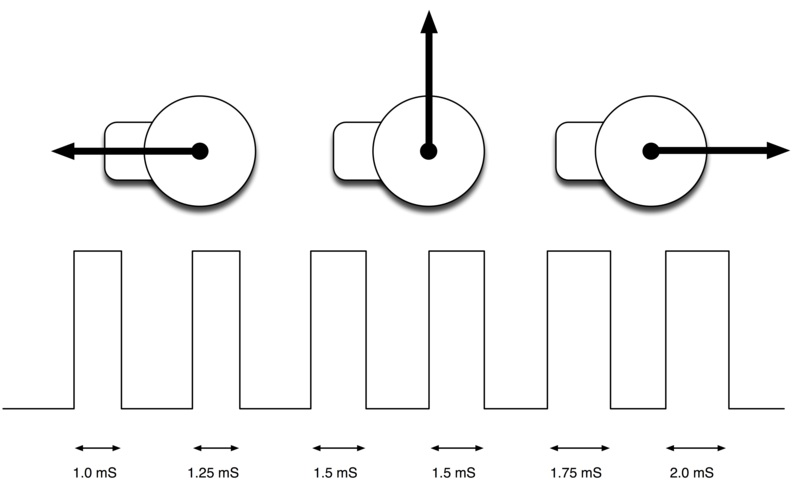
\includegraphics[width=0.79\tw]{servo-diagram.jpg}

}
\vspace{0.1in}

A sample circuit and Arduino code is shown below to get you started.
Note that the servo's ribbon wire has red, brown, and yellow wires. Red
is power, while brown is ground, and yellow is used to control the servo
from the Arduino. The \wu{470}{uF} capacitor ensures a steady power
supply to the Arduino. Make sure the longer lead of the capacitor is
connected to power while the shorter lead is connected to ground.  The
example code will sweep the servo position between 0 and 180 degrees
back and forth. After setting up the circuit and programming the
Arduino, check that the servo is sweeping back and forth steadily
between 0 and 180 degrees. You can then attach arms or horns to the
servo to control other objects and place the servo itself in more
strategic locations. Also try experimenting with smaller delays by
replacing \TT{delay(15)} with a smaller number like 5. What happens when
you try this and could it be useful?

\vspace{0.1in}
\begin{minipage}[t]{0.49\tw}
  \vspace{0.0in}
  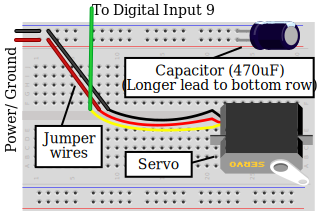
\includegraphics[width=\tw]{output-servo-annotated.svg.pdf}
\end{minipage}
\hspace{0.1in}
\begin{minipage}[t]{0.49\tw}
  \vspace{0.1in}
  \begin{Verbatim}[gobble=3,fontsize=\small]
    #include <Servo.h>

    int pin_servo = 9;

    Servo servo;
    int servo_angle = 0; // Servo position in degrees

    void setup() {
      servo.attach(pin_servo);
    }

    void loop() {
      // Scan from 0 to 180 degrees

      for( servo_angle = 0; servo_angle < 180; servo_angle++ ) {
        servo.write( servo_angle );
        delay(15);
      }

      // Scan back from 180 to 0 degrees

      for( servo_angle = 180; servo_angle > 0; servo_angle-- ) {
        servo.write( servo_angle );
        delay(15);
      }
    }
  \end{Verbatim}
\end{minipage}
\vspace{0.1in}

%Questions:

%-------------------------------------------------------------------------
% Design Project Input/Output Module Description
%-------------------------------------------------------------------------

\clearpage
\section{Piezo Output Module}
\label{sec-output-piezo}

This output module enables your IoT device to play tones using a piezo
element. A piezo element makes a clicking sound each time it is pulsed
with current. If we pulse it at the right frequency (for example 440
times a second to make the note middle A), these clicks produce notes.

A sample circuit and Arduino code is shown below to get you started.
Note that the piezo element is powered directly from the Arduino signal
pin. There is no need for any extra components; with the rectangular
"TDX" label facing to your left, we directly connect the left lead of
the piezo element to a digital output PWM pin on the Arduino and the
right lead to ground.

The example code has two experiments. In the first, we play a middle A
by pulsing the piezo element with a square wave at \wu{440}{Hz} -- i.e.,
\wu{1136}{\textmu{}s} HIGH and \wu{1136}{\textmu{}s} LOW. In the second
experiment, we play a tune using the playNote() library function. You
can use this function by giving it a note name (see the table below for
notes) and a duration to play the note; the function will play the note
using the same technique we saw in the first experiment. After setting
up the circuit and programming the Arduino, listen to the notes produced
by the piezo element and see if it makes sense. You can then experiment
with other tunes by choosing your own notes! The table below lists the
frequencies, periods, and the time to pulse the piezo element to play
different notes across two octaves.

%FIXME: The code needs to be modified to choose between experiments 1 and 2.

\vspace{0.1in}
\begin{minipage}[t]{0.49\tw}
  \vspace{0.0in}
  \centering
    \begin{tabular}{c|c|c|c}
    \BF{Note Name} & \BF{Frequency} & \BF{Period} & \BF{Time High}\\\hline
    C              & \wu{131}{Hz}   & 7634        & 3817 \\
    D              & \wu{147}{Hz}   & 6802        & 3401 \\
    E              & \wu{165}{Hz}   & 6060        & 3030 \\
    F              & \wu{175}{Hz}   & 5714        & 2857 \\
    G              & \wu{196}{Hz}   & 5102        & 2551 \\
    A              & \wu{220}{Hz}   & 4546        & 2273 \\
    B              & \wu{247}{Hz}   & 4048        & 2024 \\
    c              & \wu{261}{Hz}   & 3830        & 1915 \\
    d              & \wu{294}{Hz}   & 3400        & 1700 \\
    e              & \wu{329}{Hz}   & 3038        & 1519 \\
    f              & \wu{349}{Hz}   & 2864        & 1432 \\
    g              & \wu{392}{Hz}   & 2550        & 1275 \\
    a              & \wu{440}{Hz}   & 2272        & 1136 \\
    b              & \wu{493}{Hz}   & 2028        & 1014 \\
    \end{tabular}
  \centering

  \vspace{0.15in}
  \begin{Verbatim}[gobble=3,fontsize=\small]
    // Experiment 1: Playing a note

    #include <Piezo.h>

    int pin_piezo = 6;

    void setup() {
      pinMode( pin_piezo, OUTPUT );
    }

    void loop() {

      // Play an A4 ( 440Hz, 2272us period ).
      // Dividing the period by 2 makes 1136us --
      // the time we hold the signal HIGH or LOW.

      while (1) {
        digitalWrite( pin_piezo, HIGH );
        delayMicroseconds( 1136 );
        digitalWrite( pin_piezo, LOW );
        delayMicroseconds( 1136 );
      }
    }
  \end{Verbatim}

\end{minipage}
\hspace{0.1in}
\begin{minipage}[t]{0.49\tw}
  \vspace{0.0in}
  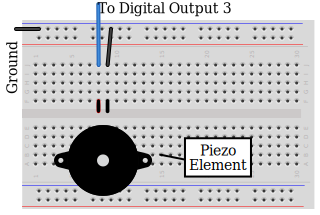
\includegraphics[width=\tw]{output-piezo-annotated.svg.pdf}

  \vspace{0.7in}
  \begin{Verbatim}[gobble=3,fontsize=\small]
    // Experiment 2: Playing a tune

    #include <Piezo.h>

    int pin_piezo = 6;

    void setup() {
      pinMode( pin_piezo, OUTPUT );
    }

    void loop() {

      // Set up the tune. The length is the
      // number of notes. The notes array
      // contains the tune -- a space is a
      // rest. The beats array contains how
      // many beats each note should take.

      int length   = 30;
      char notes[] = "ABcGGdcBAAAABcABcGGdcdeefedcdc ";
      int beats[]  = { 1, 1, 6, 1, 1, 6, 1, 1,
                       1, 1, 2, 1, 2, 6,
                       1, 1, 6, 1, 1, 6, 1, 1,
                       1, 2, 2, 1, 1, 1, 1, 4, 4 };
      int tempo    = 100;

      // Play tune using the playNote() function.

      for (int i = 0; i < length; i++) {
        playNote(pin_piezo, notes[i], beats[i] * tempo);
        delay(tempo / 2); // Pause between notes
      }

    }
  \end{Verbatim}
\end{minipage}
\vspace{0.1in}

%Questions:

%-------------------------------------------------------------------------
% Design Project Input/Output Module Description
%-------------------------------------------------------------------------

\clearpage
\section{Printer Output Module}
\label{sec-output-printer}

This printer output module enables your IoT device to print a paper copy
of collected/processed data for the end-user. The printer is a thermal
receipt printer, similar to what is in most retail stores. A thermal
printer works by selectively heating special thermochromic paper. Heated
sections of paper turn black, creating the desired text or image, such as
a barcode.

We'll be using the Arduino to control the printer. However, because the
printer's thermal print head needs to be hot to work, it requires its own
power supply. The printer comes with its own wall-wart power supply,
which you should plug into the barrel connector to screw-down terminal
converter. Ensure that positive (red) is connected to the \texttt{+} and
negative (black) is connected to the \texttt{-} as shown below:

\begin{center}
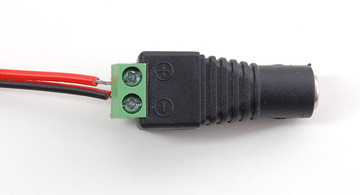
\includegraphics[width=2in]{components_poweradapt.jpg}
\end{center}

The printer has small plugs on the bottom: a 2-pin (power) and a 3-pin
(data). You'll hook up the power cable to the 2-pin plug (red/black) and
hook that up to the barrel connector converter (shown above). The data
cable connects 3-pin connector on one end and to the Arduino for control,
as shown below:

\begin{itemize}
\item Green: Digital Pin 5
\item Yellow: Digital Pin 6
\item Black: GND Pin
\end{itemize}

\begin{center}
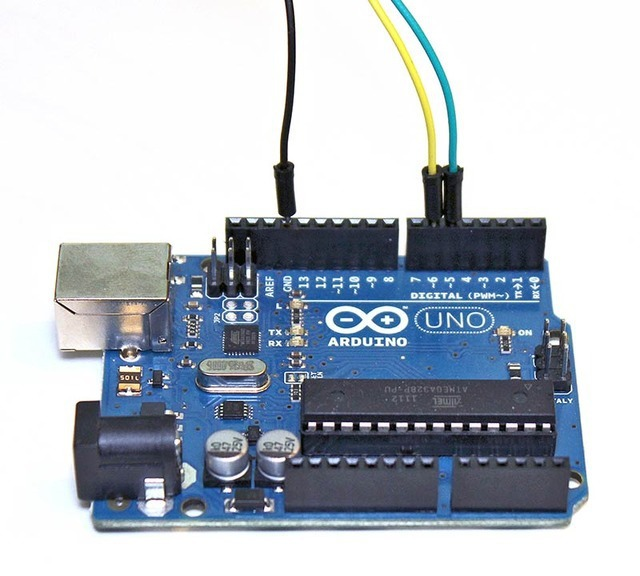
\includegraphics[width=4in]{components_printer-wiring.jpg}
\end{center}

\newpage

Using the printer is as simple as follows:

\begin{Verbatim}[gobble=3,fontsize=\small]
    #include "SoftwareSerial.h"
    #include "Adafruit_Thermal.h"
    #include <avr/pgmspace.h>

    int printer_RX_Pin = 5;  // This is the green wire
    int printer_TX_Pin = 6;  // This is the yellow wire

    Adafruit_Thermal printer(printer_RX_Pin, printer_TX_Pin);

    void setup(){
      Serial.begin(9600);
      pinMode(7, OUTPUT); digitalWrite(7, LOW); // To also work w/IoTP printer
      printer.begin();

      // The following function calls are in setup(), but do not need to be.
      // Use them anywhere!  They're just here so they're run only one time
      // and not printed over and over.
      // Some functions will feed a line when called to 'solidify' setting.
      // This is normal.

      // Hello World
      print.println("Hello World!")

      // Set text justification (right, center, left) -- accepts 'L', 'C', 'R'
      printer.justify('R');
      printer.println("This Text Right Justified");
      printer.justify('C');
      printer.println("This Text Center Justified");
      printer.justify('L');
      printer.println("This Text Left Justified");

      // Set type size, accepts 'S', 'M', 'L'
      printer.setSize('L');
      printer.println("Large Text"); // Print line
      printer.setSize('M');
      printer.println("Medium Text");
      printer.setSize('S');
      printer.println("Small Text");

      printer.feed(1);

      printer.sleep();      // Tell printer to sleep
      printer.wake();       // MUST call wake() before printing again, even if reset
      printer.setDefault(); // Restore printer to defaults
    }

    void loop() {
    }
\end{Verbatim}

%-------------------------------------------------------------------------
% Design Project Input/Output Module Description
%-------------------------------------------------------------------------

\clearpage
\section{LED Matrix Output Module}
\label{sec-output-ledmatrix}

This output module enables your IoT device to control a 16x24 LED matrix
which can display useful messages and graphics on its large screen; for
example, the matrix can display digital clocks, thermometers, counters
and meters, instrumentation readouts, industrial control indicators,
etc. You can also chain multiples of these displays together! The panel
works using a special HT1632C chip on the back which does most of the
necessary work to display messages for you. Communication with the
matrix happens through a 3-pin serial interface which is easy to work
with.

A sample circuit and Arduino code is shown below to get you started.
The LED matrix has a gray ribbon connector that has a "red strip" on one
side of it. When connecting wires to the connector, the red wire for
power will be on the same side as the "red strip" on the ribbon
connector. The example code will draw a blinking rectangle on the
screen. After setting up the circuit and programming the Arduino, check
that the shape appears on the screen correctly. You can now experiment
with drawing moving shapes or even scrolling text!

\vspace{0.1in}
\begin{minipage}[t]{0.49\tw}
  \vspace{0.0in}
  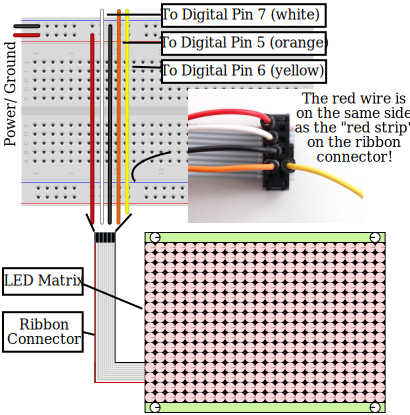
\includegraphics[width=\tw]{output-ledmatrix-annotated.svg.pdf}

\end{minipage}
\hspace{0.1in}
\begin{minipage}[t]{0.49\tw}
  \vspace{0.0in}
  \begin{Verbatim}[gobble=3,fontsize=\small]
    #include "HT1632.h"

    int pin_data = 5; // orange wire
    int pin_wr   = 6; // yellow wire
    int pin_cs   = 7; // white wire

    HT1632LEDMatrix matrix =
      HT1632LEDMatrix(pin_data, pin_wr, pin_cs);

    void setup() {
      Serial.begin(9600);
      matrix.begin(HT1632_COMMON_16NMOS);
      matrix.fillScreen();
      delay(500);
    }
  \end{Verbatim}

  \BF{RECTANGLES}:
  \vspace{0.1in}

  Use drawRect( x\_coordinate, y\_coordinate, rect\_width, rect\_height,
  value ). In this example, we draw a rectangle at point (6, 4), that
  is half the width and half the height of the entire matrix. Then we
  clear it. Use "fillRect" to draw a filled rectangle.

  \begin{Verbatim}[gobble=3,fontsize=\small]
    void loop() {
      matrix.drawRect(6, 4,
                matrix.width()/2,
                matrix.height()/2, 1);
      matrix.writeScreen();
      delay(500);
      matrix.clearScreen();
      delay(500);
    }

  \end{Verbatim}

\end{minipage}
\newpage
\begin{minipage}[t]{0.49\tw}
  \vspace{0.0in}

  \BF{PIXELS}:
  \vspace{0.1in}

  Use drawPixel( x\_coord, y\_coord, value ) In this example, we draw a
  pixel at (0, 0), delay \wu{500}{ms}, clear the pixel, and wait another
  \wu{500}{ms}.

  \begin{Verbatim}[gobble=3,fontsize=\small]
    void loop() {
      matrix.drawPixel(0, 0, 1);
      matrix.writeScreen();
      delay(500);
      matrix.drawPixel(0, 0, 0);
      delay(500);
    }
  \end{Verbatim}

  \BF{LINES}:
  \vspace{0.1in}

  Use drawLine( x1\_coordinate, y1\_coordinate, x2\_coordinate,
  y2\_coordinate, value ) In this example, we draw an X and then clear
  it.

  \begin{Verbatim}[gobble=3,fontsize=\small]
    void loop() {
      matrix.drawLine(0, 0,
                matrix.width()-1,
                matrix.height()-1, 1);
      matrix.drawLine(matrix.width()-1, 0,
                0, matrix.height()-1, 1);
      matrix.writeScreen();
      delay(500);
      matrix.clearScreen();
      delay(500);
    }
  \end{Verbatim}
\end{minipage}
\hspace{0.1in}
\begin{minipage}[t]{0.49\tw}
  \vspace{0.0in}

  \BF{CIRCLES}:
  \vspace{0.1in}

  Use \IT{drawCircle( x\_coordinate, y\_coordinate,
  radius, value )}. The coordinates are for the center of the circle. In
  this example we draw a circle and clear it. Use "fillCircle" to draw a
  filled circle instead.

  \begin{Verbatim}[gobble=3,fontsize=\small]
    void loop() {
      matrix.drawCircle(
                matrix.width()/2-1, matrix.height()/2-1,
                8, 1);
      matrix.writeScreen();
      delay(500);
      matrix.clearScreen();
      delay(500);
    }
  \end{Verbatim}

  \BF{TEXT}:
  \vspace{0.1in}

  Use:
  \begin{Verbatim}[gobble=3,fontsize=\small]
    - matrix.setCursor(x\_coordinate, y\_coordinate)
    - matrix.print( text\_to\_print )
  \end{Verbatim}

  In this example, we draw two lines of text!

  \begin{Verbatim}[gobble=3,fontsize=\small]

    void loop() {
      matrix.setTextSize(1);  // size 1 == 8 pixels high
      matrix.setTextColor(1); // 'lit' LEDs

      matrix.setCursor(0, 0); // start at top left
      matrix.print("Curi");
      matrix.setCursor(0, 8); // next line, 8 pixels down
      matrix.print("e'14");
      matrix.writeScreen();
      delay(500);
      matrix.clearScreen();
      delay(500);
    }
  \end{Verbatim}
\end{minipage}

%Questions:

%-------------------------------------------------------------------------
% Design Project Input/Output Module Description
%-------------------------------------------------------------------------

\clearpage
\section{Relay Output Module}
\label{sec-output-relay}

This output module enables your IoT device to control electrical devices
such as heaters, small skillets, lights, etc. with a signal from an
Arduino. This is ideal for making controllable lights, precision timing
cooking devices, automatic shutoff water kettles and coffee roasters,
home automation projects, or for controlling any device that plugs into
the electrical wall socket.

A sample circuit and Arduino code is shown below to get you started.
First, test the example code with the relay connected to the Arduino and
\IT{not} connected to the power strip / wall socket. Power strips / wall
sockets run at a high voltage of \wu{110}{V}, so it is good practice to
test that the circuit works with the Arduino first, which runs at a much
safer voltage of \wu{3.3--5}{V}. To connect a wire to the relay pins,
ask for a small flathead screwdriver and use it to loosen tiny screws
above each pin (turn the screw counter-clockwise to loosen), which will
open tiny wire holders in the slot below. Slip the wire into the holder
and then use the screwdriver again to tighten (turn the screw clockwise
to tighten) until the wire is steady and firm. Then program the Arduino.

The example code turns the relay on and off for {5}{s} each in a loop.
After programming the Arduino, you should see the LED turn on and off
for {5}{s}. The LED indicates when the device under control is receiving
power. If this works, you can plug one end of the relay into a power
strip / wall socket, and you can plug an appliance (e.g., a mini-fan)
into the other end. Turn the fan on and make sure it is on for {5}{s}
and off for {5}{s}. Try experimenting with other devices and see what
you can control! Modify the {5}{s} looped Arduino code if you want to
control timing in other ways.

\vspace{0.1in}
\begin{minipage}[t]{0.49\tw}
  \vspace{0.0in}
  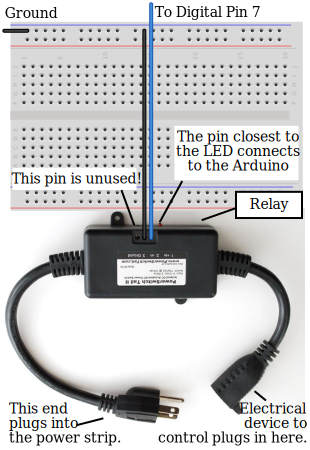
\includegraphics[width=\tw]{output-relay-annotated.svg.pdf}
\end{minipage}
\hspace{0.1in}
\begin{minipage}[t]{0.49\tw}
  \vspace{0.1in}
  \begin{Verbatim}[gobble=3,fontsize=\small]
    int pin_relay = 7;

    void setup() {
      pinMode( pin_relay, OUTPUT );
    }

    void loop() {
      digitalWrite( pin_relay, HIGH );
      delay(5000);
      digitalWrite( pin_relay, LOW );
      delay(5000);
    }
  \end{Verbatim}
\end{minipage}
\vspace{0.1in}

%Questions:


\end{document}

